\documentclass[hidelinks, a4paper, 12pt]{article}
\usepackage[linktoc=all]{hyperref}
\usepackage{apacite}
\usepackage[margin=1.0in]{geometry}
\usepackage{amssymb}
\usepackage{amsmath}
\usepackage{amsthm}
\usepackage{pgfplots}
\usepackage{tikz}
\usepackage{pgf}
\usepackage{mathrsfs}

% \makeatletter
% \renewcommand{\@dotsep}{10000} 
% \makeatother

\hypersetup{
    pdftitle={Pure Mathematics III: Vectors},
    pdfauthor={Wilson Wongso},
    pdfpagemode=UseOutlines,
}

\usetikzlibrary{arrows}
\pgfplotsset{compat=1.16}

\title{Pure Mathematics III: Vectors}
\author{Based on lectures by Danilo J. Alcordo \\ Notes taken by Wilson Wongso}
\date{Junior College 2 - Academic Year 2018/2019}

\setcounter{section}{-1}
\setcounter{tocdepth}{2}

\graphicspath{ {./images/} }

\newcommand{\bd}{\textbf}
\newcommand{\biimp}{\Leftrightarrow}
\newcommand{\thus}{\Rightarrow}
\newcommand{\nhat}{\hat{n}}
\newcommand{\mhat}{\hat{m}}
\newcommand{\uhat}{\hat{u}}
\newcommand{\vhat}{\hat{v}}
\newcommand{\n}{\\[\baselineskip]}
\newcommand{\ceq}{\overset{?}{=}}

\begin{document}
    \maketitle
    
    \tableofcontents

    \section{Preface}
        The following lecture notes are mostly based on textbook \cite{neill2016cambridge} questions and past-paper questions from various years.
        The author assumes that the readers are able to do basic vector operations and understands coordinate geometry.\\[\baselineskip]
        These notes only include the key parts of the lectures and the types of problems that often appear in the actual exam.
        Further reading and past-year papers practice are highly encouraged.
    
    \section{Vector Equations}
        \subsection{Introduction}
            Point on a line through $\bd{a}$ in the direction of $\textbf{p}$ have position vectors $\textbf{r} = \textbf{a} + t\textbf{p}$, where $t$ is a
            variable scalar. This is called the \textbf{vector equation} of a line.\\[\baselineskip]
            Lines with vector equation $\textbf{r} = \textbf{a} + t\textbf{p}$ and $\textbf{r} = \textbf{b} + t\textbf{q}$ have the same direction if \textbf{$p$}
            is a multiple of $\textbf{q}$. If in addition, $\textbf{b} - \textbf{a}$ is a multiple of $\textbf{q}$, the lines are the same; otherwise the lines
            are parallel.
        
        \subsection{Vector Equation from a Point and a Directional Vector}
            With a given point $p$ and a directional vector $\hat{n}$, we can form the vector equation:
            \[r = p + \lambda \nhat\]
            as well as obtain both parametric and Cartesian equations.
            \subsubsection{Example 1}
                Given the point $p (2, -3)$ and $\nhat = $
                $\begin{pmatrix}
                    1 \\ 
                    2
                \end{pmatrix}$,
                find its vector equation, parametric equations, and Cartesian equation.\n
                \bd{Solution}\\
                Vector Equation:
                \[r = \begin{pmatrix} 2 \\ -3 \end{pmatrix} + \lambda \begin{pmatrix} 1 \\ -3 \end{pmatrix}\]
                \[r = \begin{pmatrix} 2 \\ -3 \end{pmatrix} + \begin{pmatrix} \lambda \\ -3\lambda \end{pmatrix}\]
                \[r = \begin{pmatrix} 2 + \lambda \\ -3-3\lambda \end{pmatrix}\]
                Parametric Equations:
                \begin{equation}
                    x = 2 + \lambda
                \end{equation}
                \begin{equation}
                    y = -3 - 3\lambda  
                \end{equation}
                Cartesian Equation:\n
                Make $\lambda$ the subject of equation $(1)$: 
                \begin{equation}
                    \lambda = x - 2
                \end{equation}
                Substitute equation $(3)$ into equation $(2)$:
                \[y = -3 - 3(x-2)\]
                \[y = -3 -3x + 6\]
                Obtaining:
                \[y = -3x + 3\]
                as our Cartesian equation.
            \subsubsection{Example 2}
                Given that the line passes through origin and is parallel to $\nhat = $
                $\begin{pmatrix}
                    -2 \\ 
                    3
                \end{pmatrix}$,
                find its vector equation, parametric equations, and Cartesian equation.\n
                \bd{Solution}\\
                Vector Equation:
                \[r = \begin{pmatrix} 0 \\ 0 \end{pmatrix} + \lambda \begin{pmatrix} -2 \\ 3 \end{pmatrix}\]
                \[r = \begin{pmatrix} -2\lambda \\ 3\lambda \end{pmatrix}\]
                Parametric Equations:
                \begin{equation}
                    x = -2\lambda
                \end{equation}
                \begin{equation}
                    y = 3\lambda  
                \end{equation}
                Cartesian Equation:\n
                Make $\lambda$ the subject of equation $(3)$: 
                \begin{equation}
                    \lambda = -\frac{1}{2}x 
                \end{equation}
                Substitute equation $(6)$ into equation $(5)$:
                \[y = 3\left(-\frac{1}{2}x\right)\]
                Obtaining:
                \[y = -\frac{3}{2}x\]
                as our Cartesian equation.
            \subsubsection{Example 3}
                Find the vector equation for lines with the following Cartesian equation:
                \[x + 3y = 7\]
                \bd{Solution}\\
                Rearrange the Cartesian to be of the form $y = mx + c$:
                \[3y = -x + 7\]
                \[y = -\frac{1}{3}x + \frac{7}{3}\]
                \bd{Notice: }$m = -\frac{1}{3}$, and as we know:
                \[m = \frac{\Delta y}{ \Delta x} = -\frac{1}{3}\]
                Hence in its directional vector form, denoted by $\nhat$:
                \[\nhat = \begin{pmatrix} \Delta x\\\Delta y \end{pmatrix} = \begin{pmatrix} 3\\-1 \end{pmatrix}\]
                Then, to find one point that passes through the line, we can set $x$ to any value. For instance, when:
                \[x = 1\]
                We find:
                \[y = -\frac{1}{3} + \frac{7}{3} \]
                \[y = \frac{6}{3}\]
                \[y = 2\]
                Thus obtaining point at $(1, 2)$, with which we can form the vector equation:
                \[r = \begin{pmatrix} 1 \\ 2 \end{pmatrix} + \lambda \begin{pmatrix} 3 \\ -1 \end{pmatrix}\]
            \subsubsection{Example 4}
                Find the vector equation for lines with the following Cartesian equation:
                \[x = 2\]
                \bd{Solution}\\
                Unlike \bd{1.2.3 Example 3}, our line has no $y$ in its equation, and if we notice:
                \begin{figure}[!ht]
                    \centering
                    \begin{tikzpicture}
                            \begin{axis}[ 
                            xmin=-1, xmax=3,
                            ymin=-1, ymax=3,
                            axis lines=middle,
                            xlabel=$x$,
                            ylabel={$y$}
                        ] 
                        \addplot +[mark=none, color=red] coordinates {(2, -1) (2, 3)};
                            \legend{x=2}
                        \end{axis}  
                    \end{tikzpicture}
                \end{figure}\n
                The line $x = 2$ is a straight, vertical line, whose gradient is undefined! If we try to calculate it:
                \[m = \frac{a}{0} = undefined,\]
                where $a$ is a constant. Thus, its directional vector is:
                \[\nhat = \begin{pmatrix} 0 \\ 1 \end{pmatrix}\]
                \bd{Note: }We chose $1$ as our value to $a$, but it can be any other constant, because any value of $a$
                will still make the gradient be undefined.\n
                Therefore, the vector equation formed by the line is:
                \[r = \begin{pmatrix} 2 \\ 0 \end{pmatrix} + \lambda \begin{pmatrix} 0 \\ 1 \end{pmatrix}\]
        \subsection{Vector Equation from two Points of a Line}
            With given points $p$ and $q$, we can form the vector equation:
            \[r = p + \lambda\nhat\]
            or,
            \[r = q + \lambda\nhat\]
            where:
            \[\nhat = p - q\]
            or,
            \[\nhat = q - p\]
            \subsubsection{Example 1}
                Given that a line passes through the point $p (0, 7)$ and $q (5, 0)$,
                find its vector equation and its parametric equations.\n
                \bd{Solution}\\
                Vector Equation:
                \[r = \begin{pmatrix} 0 \\ 7 \end{pmatrix} + \lambda\begin{pmatrix} 5-0 \\ 0-7 \end{pmatrix}\]
                \[r = \begin{pmatrix} 0 \\ 7 \end{pmatrix} + \lambda\begin{pmatrix} 5 \\ -7 \end{pmatrix}\]
                \[r = \begin{pmatrix} 0 \\ 7 \end{pmatrix} + \begin{pmatrix} 5\lambda \\ -7\lambda \end{pmatrix}\]
                \[r = \begin{pmatrix} 5\lambda \\ 7-7\lambda \end{pmatrix}\]
                Parametric Equations:
                \[\begin{split}
                    x &= 5\lambda\\
                    y &= 7 - 7\lambda
                \end{split}\]
        \subsection{Point of Intersection between two Vector Equations}
            Given two vector equations $r_1$ and $r_2$, we can equate both of them:
            \[r_1 = r_2\]
            and solve the system of linear equations to obtain the point of intersection.
            \subsubsection{Example 1}
                Find the coordinate of the points common to the following pair of lines, if any.
                \[r_1 = \begin{pmatrix} 2 \\ 0 \end{pmatrix} + \lambda \begin{pmatrix} 5 \\ 3 \end{pmatrix}\]
                \[r_2 = \begin{pmatrix} 3 \\ -1 \end{pmatrix} + \mu \begin{pmatrix} 1 \\ 1 \end{pmatrix}\]
                \bd{Solution}
                \[r_1 = r_2\]
                \[\begin{pmatrix} 2 + 5 \lambda \\ 3 \lambda \end{pmatrix} = \begin{pmatrix} 3 + \mu \\ -1 + \mu \end{pmatrix} \]
                From which we get:
                \begin{equation}
                    \begin{split}
                        \thus 2 + 5 \lambda &= 3 + \mu\\
                        5 \lambda - \mu &= 1
                    \end{split}
                \end{equation}
                and:
                \[3 \lambda = -1 + \mu\]
                \begin{equation}
                    3\lambda - \mu = - 1
                \end{equation}
                Subtracting both sides of equation $(7)$ and $(8)$ respectively yields:
                \[2\lambda = 2\]
                \[\lambda = 1\]
                With the value of $\lambda$, we can substitute it into $r_1$:
                \[r_1 = \begin{pmatrix} 2 + 5 \\ 3 \end{pmatrix}\] 
                \[r_1 = \begin{pmatrix} 7 \\ 3 \end{pmatrix}\]
                Hence the point of intersection being:
                \[(7, 3)\]
                \bd{Note: }Solving for the value of $\mu$ and substituting it into $r_2$ will also yield the same result.
            \subsubsection{Example 2}
                Find the coordinate of the points common to the following pair of lines, if any.
                \[r_1 = \begin{pmatrix} 2 \\ -1 \end{pmatrix} + \lambda \begin{pmatrix} 1 \\ -3 \end{pmatrix}\]
                \[r_2 = \begin{pmatrix} 4 \\ 0 \end{pmatrix} + \mu \begin{pmatrix} -2 \\ 6 \end{pmatrix}\]
                \bd{Notice: }
                \[\begin{pmatrix} -2 \\ 6 \end{pmatrix} = -2 \begin{pmatrix} 1 \\ -3 \end{pmatrix}\]
                \[\thus \nhat_2 = a \nhat_1\]
                where $a$ is a scalar. Since the directional vector $\nhat_2$ is a multiple of $\nhat_1$, that means
                both lines are parallel to each other (See \bd{1.1 Introduction}). And from coordinate geometry, we know that two parallel lines never
                intersect each other. Hence, there are no common points.
            \subsubsection{Example 3}
                Find the coordinate of the points common to the following pair of lines, if any.
                \[r_1 = \begin{pmatrix} 7 \\ 1 \end{pmatrix} + \lambda \begin{pmatrix} 6 \\ -4 \end{pmatrix}\]
                \[r_2 = \begin{pmatrix} 10 \\ -1 \end{pmatrix} + \mu \begin{pmatrix} -9 \\ 6 \end{pmatrix}\]
                \bd{Notice: }
                \[2\begin{pmatrix} 3 \\ -2 \end{pmatrix} = -3 \begin{pmatrix} 3 \\ -2 \end{pmatrix}\]
                \[\thus a\begin{pmatrix} 3 \\ -2 \end{pmatrix} = b \begin{pmatrix} 3 \\ -2 \end{pmatrix}\]
                where $a$ and $b$ are scalars, and $\nhat_1$ and $\nhat_2$ are multiples of $\begin{pmatrix} 3 \\ -2 \end{pmatrix}$.\n
                In addition:
                \[\begin{pmatrix} 10 \\ -1 \end{pmatrix} - \begin{pmatrix} 7 \\ 1 \end{pmatrix} = \begin{pmatrix} 3 \\ -2 \end{pmatrix}\]
                \[\begin{pmatrix} 3 \\ -2 \end{pmatrix} = \begin{pmatrix} 3 \\ -2 \end{pmatrix}\]
                \[\thus p_2 - p_1 = a\begin{pmatrix} 3 \\ -2 \end{pmatrix}\]
                with $a$ having the value of $1$.\n
                Similar to \bd{1.4.2 Example 2}, $r_1$ and $r_2$ are not only parallel lines, but also are the exact same lines. Thus, there are
                no common points.
    
    \section{Vector Equations in 3-Dimensions}
        \subsection{Introduction}
            Unlike in 2-Dimensions, 3-Dimension Vector Equation deals with 3 coordinates, usually denoted by $x$, $y$, and $z$.
            Later on, we can form vector equation of a line in 3-dimensions, as well as vector equation of a plane. Since we are dealing with 3 coordinates, 
            we move on to vectors with 3 elements:
            \[\begin{pmatrix} x \\ y \\ z \end{pmatrix}\]
            Methods such as to find vector equation from a point and a directional vector, point of intersection, etc., still works the same in 3-D.\n
            Similarly, methods to be introduced also works in 2-D, but for future convenience we are going to start using 3-D.
        
        \subsection{Finding out whether a Point lies on a Line}
            Given the point $p_1(x, y, z)$ that lies on a vector equation $r = p_0 + \lambda \nhat$, we can find a value of $\lambda$ that satisfies the equation:
            \[p_1 = p_0 + \lambda \nhat\]
            \subsubsection{Example 1}
                Find whether or not the point $p(-3, 1, 5)$ lies on the following line:
                \[r = \begin{pmatrix} 1 \\ 3 \\ 1 \end{pmatrix} + \lambda \begin{pmatrix} -2 \\ -1 \\ 2 \end{pmatrix}\]
                \bd{Solution:}
                \[\begin{pmatrix} -3 \\ 1 \\ 5 \end{pmatrix} = \begin{pmatrix} 1 \\ 3 \\ 1 \end{pmatrix} + \lambda \begin{pmatrix} -2 \\ -1 \\ 2 \end{pmatrix}\]
                \[\lambda \begin{pmatrix} -2 \\ -1 \\ 2 \end{pmatrix} = \begin{pmatrix} -3 \\ 1 \\ 5 \end{pmatrix} - \begin{pmatrix} 1 \\ 3 \\ 1 \end{pmatrix}\]
                \[\lambda \begin{pmatrix} -2 \\ -1 \\ 2 \end{pmatrix} = \begin{pmatrix} -4 \\ -2 \\ 4 \end{pmatrix}\]
                We find that:
                \[\lambda = 2\]
                satisfies the equation. Thus the point $p$ lies on line $r$.
            \subsubsection{Example 2}
                Find whether or not the point $p(-3, 1, 5)$ lies on the following line:
                \[r = \begin{pmatrix} 0 \\ 1 \\ 2 \end{pmatrix} + \lambda \begin{pmatrix} 1 \\ 0 \\ 3 \end{pmatrix}\]
                \bd{Solution:}
                \[\begin{pmatrix} -3 \\ 1 \\ 5 \end{pmatrix} = \begin{pmatrix} 0 \\ 1 \\ 2 \end{pmatrix} + \lambda \begin{pmatrix} 1 \\ 0 \\ 3 \end{pmatrix}\]
                \[\lambda \begin{pmatrix} 1 \\ 0 \\ 3 \end{pmatrix} = \begin{pmatrix} -3 \\ 1 \\ 5 \end{pmatrix} - \begin{pmatrix} 0 \\ 1 \\ 2 \end{pmatrix}\]
                \[\lambda \begin{pmatrix} 1 \\ 0 \\ 3 \end{pmatrix} = \begin{pmatrix} -3 \\ 0 \\ 3 \end{pmatrix}\]
                We find that no value of $\lambda$ will satisfy the equation. Thus point $p$ does not lie on line $r$.

        \subsection{Cross Product}
            In order to be able to do further calculations, we need to first understand another operator for vectors, the cross product. Unlike the dot product, the cross
            product requires both of the vectors to be in 3-dimensions. The operator is denoted by:
            \[\hat{u}\times\hat{v}\]
            While the dot product of two vectors returns a scalar, the cross product returns another vector which is orthogonal to both input vectors.
            \subsubsection{Finding the Cross Product}
                Given the vector:
                \[\hat{u} = \begin{pmatrix} x \\ y \\ z \end{pmatrix}\]
                and the vector:
                \[\hat{v} = \begin{pmatrix} \alpha \\ \beta \\ \gamma \end{pmatrix}\]
                Hence their cross product is:
                \[
                    \begin{split}
                        \hat{u}\times\hat{v} &= \begin{pmatrix} x \\ y \\ z \end{pmatrix} \times \begin{pmatrix} \alpha \\ \beta \\ \gamma \end{pmatrix}\\
                        \hat{u}\times\hat{v} &= \begin{pmatrix} y\gamma - z\beta \\ z\alpha - x\gamma \\ x\beta - y\alpha \end{pmatrix}\\
                    \end{split}
                \]
                It's pretty difficult to memorize the cross product by its formula. The author found a simpler and more intuitive method to finding the cross product.\n
                Given the same vectors $\hat{u}$ and $\hat{v}$, list out the components of each vector with respect to the unit vectors $i$, $j$ and $k$:
                \begin{center}
                    \begin{tabular}{|c || c | c | c|} 
                    \hline
                    Vector & $i$ & $j$ & $k$ \\
                    \hline
                    $\hat{u}$ & $x$ & $y$ & $z$ \\ 
                    \hline
                    $\hat{v}$ & $\alpha$ & $\beta$ & $\gamma$ \\
                    \hline
                   \end{tabular}
                \end{center}
                Then, the $i$ component of the cross product is the determinant of the matrix:
                \[A = \begin{pmatrix} y & z \\ \beta & \gamma \end{pmatrix}\]
                \[det(A) = y\gamma - z\beta\]
                \bd{Notice: } $A$ is simply the matrix formed when column $i$ is covered up from the table.\n
                Similarly, the $j$ component of the cross product is the \bd{negative} of the determinant of the matrix formed when column $j$ is covered up:
                \[B = \begin{pmatrix} x & z \\ \alpha & \gamma \end{pmatrix}\]
                \[\begin{split}
                    det(B) &= x\gamma - z\alpha\\
                    \thus -det(B) &= z\alpha - x\gamma
                \end{split}\]
                Lastly, the $k$ component of the cross product is the determinant of the matrix formed when column $k$ is covered up:
                \[C = \begin{pmatrix} x & y \\ \alpha & \beta \end{pmatrix}\]
                \[det(C) = x\beta - y\alpha\]
                Therefore, the cross product is equivalent to:
                \[\hat{u}\times\hat{v} = det(A)i - det(B)j + det(C)k\]
                \[\hat{u}\times\hat{v} = (y\gamma - z\beta)i - (x\gamma - z\alpha)j + (x\beta - y\alpha)k\]
                \[\hat{u}\times\hat{v} = (y\gamma - z\beta)i + (z\alpha - x\gamma)j + (x\beta - y\alpha)k\]
                which yields the same results as the formula of the cross product.
        
    \section{Plane Equations}
        Now that we've entered 3-dimensions, we are no longer bounded by lines - instead planes. And just like lines, planes too have their vector equations.
        \subsection{Introduction}
            Normally, a line is described with the vector uniquely parallel to it, usually denoted by $\nhat$.\n
            With planes, there are many \bd{pairs} of vectors \bd{parallel} to the it, but there exists a vector which is uniquely \bd{normal} or \bd{orthogonal} to it.
            This normal vector is used to determine a plane, usually denoted by $\mhat$.
        
        \subsection{Normal Equation of a Plane}
            Let $\mhat$ be a vector normal to a plane. Let $r$ be a position vector of a point on the plane, and $a$ be any other point on the plane.
            \begin{figure}[ht]
                \centering
                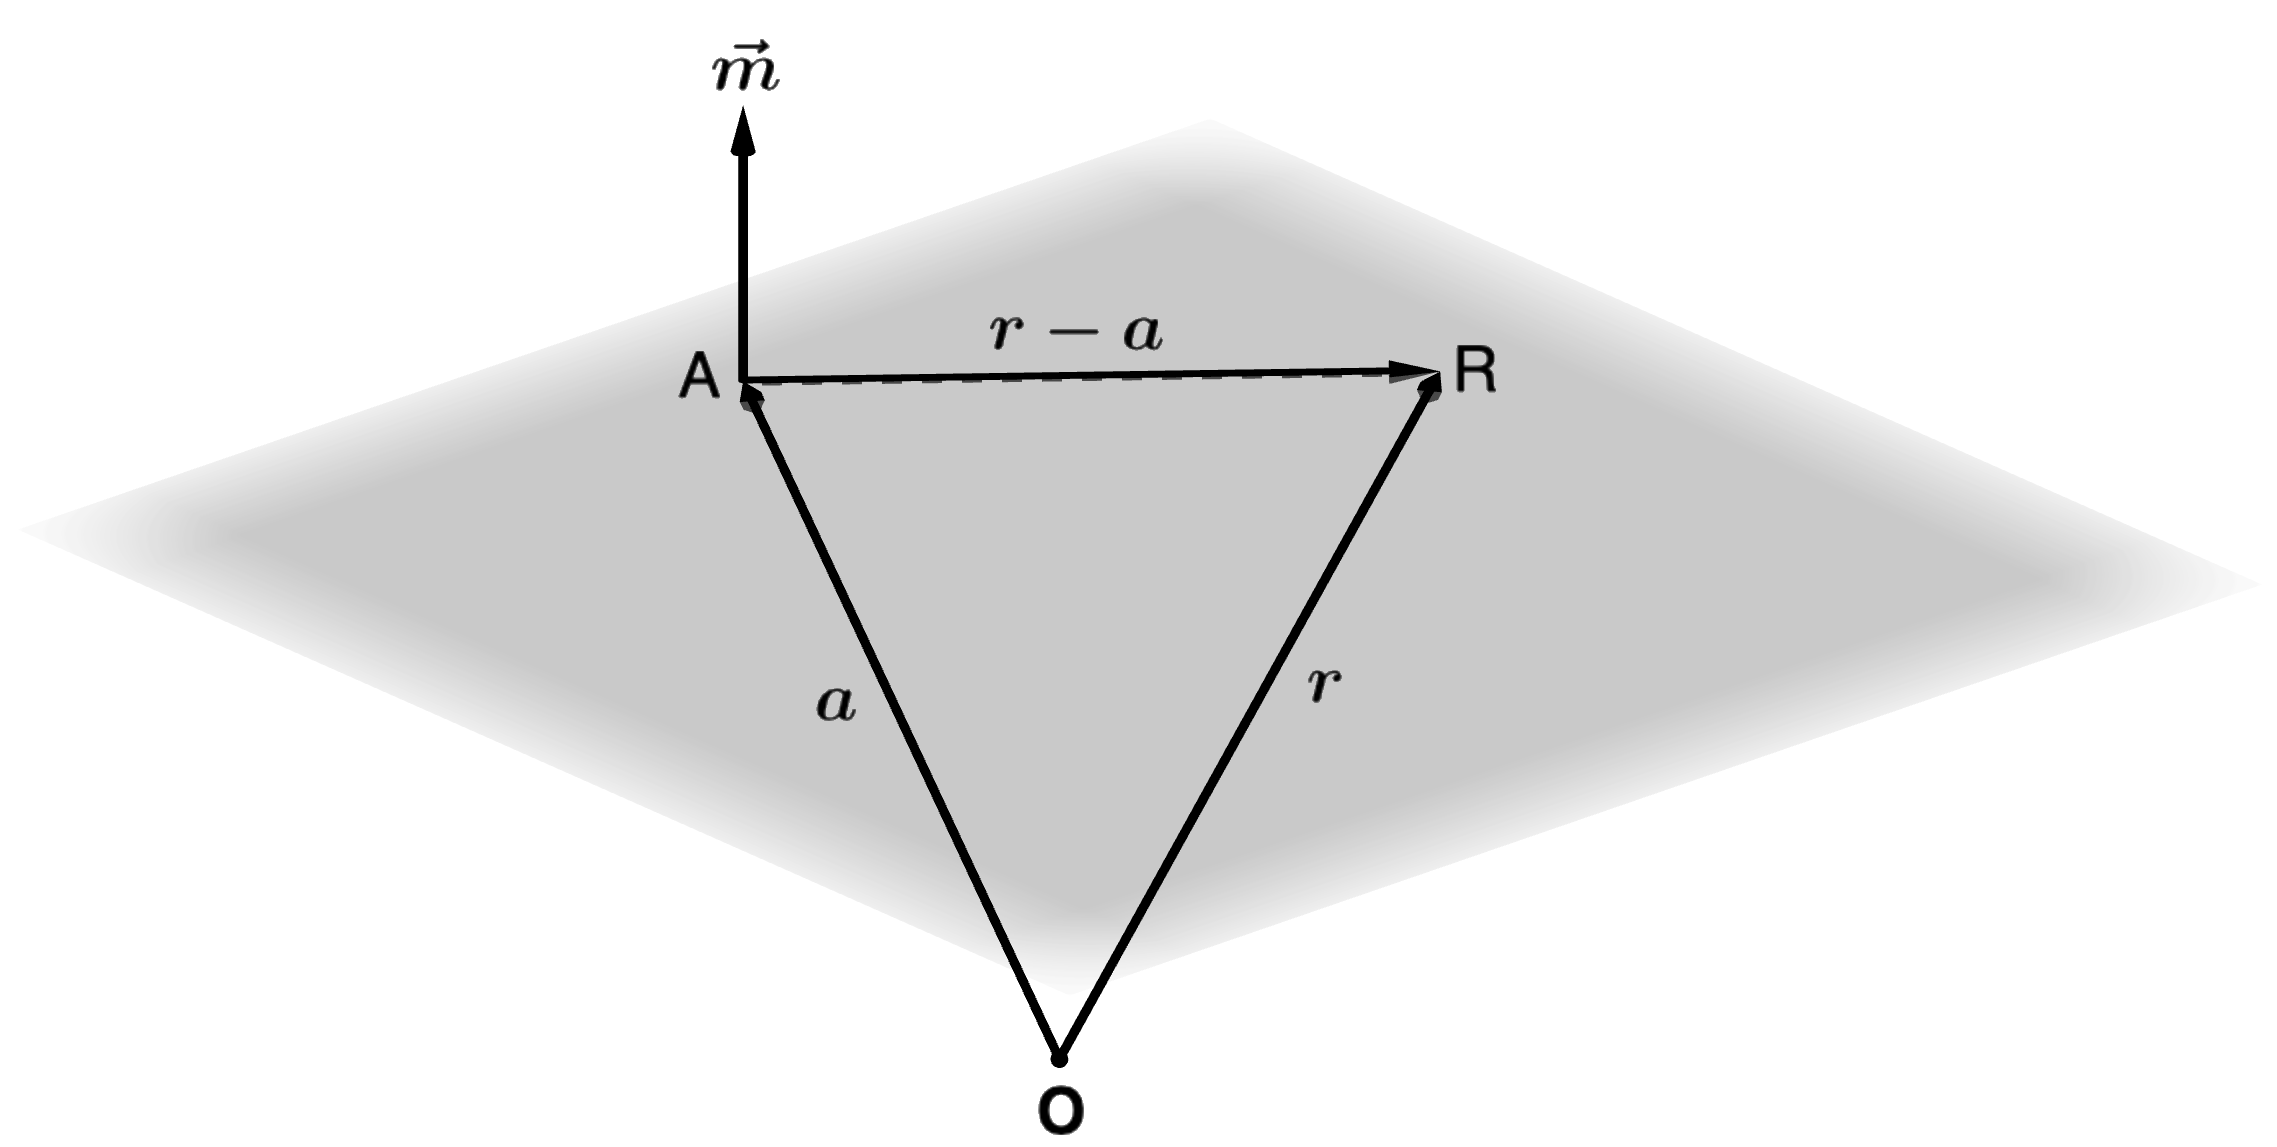
\includegraphics[width=10cm, height=5cm]{normal-equation}       
            \end{figure}\\
            Then the vector $r-a$ is a vector parallel to the plane, and is therefore normal to $\mhat$.\\
            Thus, the plane has the normal equation:
            \[(r-a) \cdot \mhat = 0\]
            or equivalently,
            \begin{equation}
                r \cdot \mhat = a \cdot \mhat
            \end{equation}  
            
        \subsection{Cartesian Equation of a Plane}
            If we write $r = \begin{pmatrix}x\\y\\z\end{pmatrix}$ and $\mhat = \begin{pmatrix}a\\b\\c\end{pmatrix}$, equation $(9)$ becomes of the form:
            \[ax + by + c = a\cdot\mhat\]
            And the right hand side of the equation is just a constant. Therefore, the plane has the Cartesian Equation:
            \[ax + by + c = d\]
            where $d$ is a constant determined by the coordinates of $a$.
            \subsubsection{Example 1}
                Find the Cartesian equation of a plane that passes through the point $p(2, -4, -5)$ and is perpendicular to the vector $3i + j - 2k$.\n
                \bd{Solution}\\
                Let $r = \begin{pmatrix}x\\y\\z\end{pmatrix}$, and $\mhat = \begin{pmatrix}3\\1\\-2\end{pmatrix}$, then the plane has the Cartesian equation:
                \[r\cdot\mhat = d\]
                \begin{equation}
                    \begin{pmatrix} x\\y\\z \end{pmatrix} \cdot \begin{pmatrix} 3\\1\\-2 \end{pmatrix} = d
                \end{equation}
                In order to find the value of $d$ that satisfies the point $p$, we need to substitute the values of $x$, $y$ and $z$ in equation $(10)$ by the coordinates of $p$,
                \[\begin{pmatrix} 2\\-4\\-5 \end{pmatrix} \cdot \begin{pmatrix} 3\\1\\-2 \end{pmatrix} = d\]
                \[6-4+10 = d\]
                \[d = 12\]
                With that, our equation $(10)$ becomes
                \[\begin{pmatrix} x\\y\\z \end{pmatrix} \cdot \begin{pmatrix} 3\\1\\-2 \end{pmatrix} = 12\]
                And our Cartesian equation as the final answer is:
                \[3x + y - 2z = 12\]
        
        \subsection{Vector Equation of a Plane from 3 Points on the Plane}
            As said in \bd{3.1 Introduction}, we can use a pair of vectors parallel to the plane to describe the plane's equation. Given three points $A$, $B$,
            and $C$ that lies on a plane, then the plane has the vector equation:
            \[r = \vec{OA} + \lambda (\vec{AB}) + \mu (\vec{AC})\]
            where $O$ is the origin, both $\lambda$ and $\mu$ being variable scalars.\n
            \bd{Note: }You can interchange $\vec{OA}$ with $\vec{OB}$ or $\vec{OC}$, since all three of them lies on the plane.
            Likewise, you can vary the vectors $\vec{AB}$ and $\vec{AC}$ with any two of the three points, since the vectors formed will all be parallel to the plane. However,
            the two vectors have to be distinct to one another.

    \section{Distance}
        The concept of distance will be used again in Vectors in Pure Mathematics III. However, they will be in a deeper level, where we can find the distance from various
        quantities, such as from point-to-line distance, line-to-line distance, point-to-plane distance, plane-to-plane distance, etc.
        \subsection{Magnitude of a Vector}
            From Vectors in Pure Mathematics I, we know that a vector has its respective magnitude, which corresponds to the quantity distance from a point to another.
            The equation we used in 2-D is similar to that of Pythagoras' Theorem, where the vector:
            \[\hat{a} = \begin{pmatrix} x \\ y \end{pmatrix}\]
            has a magnitude of:
            \[|\hat{a}| = \sqrt{x^2 + y^2}\]
            And unsurprisingly, the equation still holds for vectors in 3-dimensions, where the vector:
            \[\hat{a} = \begin{pmatrix} x \\ y \\ z \end{pmatrix}\]
            has a magnitude of:
            \[|\hat{a}| = \sqrt{x^2 + y^2 + z^2}\]

        \subsection{Distance from a Point to a Line}
            There are two methods taught in order to find the distance from a point to a line, one utilizing a distance equation, and the other
            being a more intuitive approach. The more formal approach has the equation:
            \[dis(p, r) = \frac{|\vec{pp_0}\times \nhat|}{|\nhat|}\]
            where, $r = p_0 + \lambda \nhat$ is the vector equation of the line and $p$ is a point in space.\n
            The more informal method might be easier to be understood via an example problem, as follows:
            \subsubsection{Example 1}
                Calculate the distance of the point $p(-6, 1, 21)$ to the line $r = \begin{pmatrix} -4\\-5\\-1 \end{pmatrix} + \mu\begin{pmatrix} 3\\1\\1 \end{pmatrix}$.\\
                \bd{Solution}\\
                Firstly, we let a point $p'$ be a point on the line $r$, which is the foot of the perpendicular from the point $p$ to $r$.
                \begin{tikzpicture}[line cap=round,line join=round,>=triangle 45,x=1cm,y=1cm]
                    \clip(0.5455830571350128,-2.635019050122706) rectangle (11.118226510324153,3.7069303896772774);
                    \draw [->,line width=0.8pt] (1,0) -- (9,0);
                    \draw [line width=0.8pt] (3,3)-- (3,0);
                    \draw [line width=0.8pt] (3.1434138353075785,0.15327340430840822)-- (3.1434138353075785,0);
                    \draw [line width=0.8pt] (3.1434138353075785,0.15327340430840822)-- (3,0.15327340430840808);
                    \draw (2.910516461137847,-0.01640766852787435) node[anchor=north west] {$p'$};
                    \draw (9.080619529020673,0.1881713456592219) node[anchor=north west] {$r$};
                    \draw (3.010516461137847,3.4287029303828263) node[anchor=north west] {$p$};
                    \begin{scriptsize}
                    \draw [fill=black] (3,3) circle (1pt);
                    \draw [fill=black] (3,0) circle (1pt);
                    \end{scriptsize}
                \end{tikzpicture}\n
                In that case, as the point $p'$ lies on the line $r$, it has the general equation of r, but still with an unknown value of $\mu$:
                \[p' = \begin{pmatrix} -4\\-5\\-1 \end{pmatrix} + \mu\begin{pmatrix} 3\\1\\1 \end{pmatrix}\] 
                Then, we find the vector $\vec{pp'}$:
                \[\begin{split}
                    \vec{pp'} &= p' - p \n
                    \vec{pp'} &= \begin{pmatrix} -4\\-5\\-1 \end{pmatrix} + \mu\begin{pmatrix} 3\\1\\1 \end{pmatrix} - \begin{pmatrix} -6\\1\\21 \end{pmatrix}\n 
                    \vec{pp'} &= \begin{pmatrix} 3\mu + 2 \\ \mu - 6\\ \mu -22\end{pmatrix}                       
                \end{split}\]
                And as we can see from the diagram, $\vec{pp'}$ is orthogonal to the directional vector of $r$, $\nhat$. Hence:
                \begin{equation}\vec{pp'}\cdot \nhat = 0\end{equation}
                From which we can find the value of $\mu$ that satisfies equation $(11)$.
                \[\thus\begin{pmatrix} 3\mu + 2 \\ \mu - 6\\ \mu -22\end{pmatrix} \cdot \begin{pmatrix} 3\\1\\1 \end{pmatrix} = 0\]
                \[9\mu + 6 + \mu - 6 + \mu - 22 = 0\]
                \[11\mu = 22\]
                \[\mu = 2\]
                With the actual value of $\mu$ for the point $p'$, we can substitute it to the vector $\vec{pp'}$:
                \[\begin{split}
                    \vec{pp'} &= \begin{pmatrix} 3\mu + 2 \\ \mu - 6\\ \mu -22\end{pmatrix}\\
                    \vec{pp'} &= \begin{pmatrix} 6 + 2 \\ 2 - 6\\ 2 -22\end{pmatrix}\\
                    \vec{pp'} &= \begin{pmatrix} 8 \\ -4 \\ -20\end{pmatrix}
                \end{split}\]
                And, if you haven't noticed, the magnitude of $\vec{pp'}$ is the distance of the point $p$ to the line $r$ -- the value we've been looking for all along.
                \[|\vec{pp'}| = \sqrt{(8)^2 + (-4)^2 + (-20)^2}\]
                \[\begin{split}
                    |\vec{pp'}| &= \sqrt{480}\\
                    |\vec{pp'}| &= \sqrt{16*30}\\
                    |\vec{pp'}| &= 4\sqrt{30}\\
                    \thus dis(p, r) &= 4\sqrt{30}
                \end{split}\]
                \bd{Note: }Using the formula for distance between point and line would yield the same result.
            
        \subsection{Distance from a Line to another Line}
            The equation to find the distance between two lines is very similar to that of a point to a line. However, it involves
            using the cross product, which we've discussed before in \bd{2.3 Cross Product}. Since it uses the cross product,
            the lines have to be in 3-dimensions. It is as follows:
            \[dis(r_1, r_2) = \frac{|(\vec{PQ}) \cdot (\hat{u} \times \hat{v})|}{|\hat{u} \times \hat{v}|}\]
            where, $r_1 = Q + \lambda \hat{u}$ and $r_2 = P + \mu \hat{v}$.\n
            \bd{Note: }The dot product in the numerator produces a scalar, hence the value taken is its absolute value. On the other hand, the denominator corresponds to the magnitude
            of the cross product of the two directional vectors of the respective lines.
            \subsubsection{Example 1}
                Find the shortest distance between two skew lines\n
                $r_1 = \begin{pmatrix} 0\\2\\-1 \end{pmatrix} + \mu\begin{pmatrix} 1\\1\\2 \end{pmatrix}$ and
                $r_2 = \begin{pmatrix} 1\\0\\-1 \end{pmatrix} + \lambda\begin{pmatrix} 1\\1\\3 \end{pmatrix}$\n
                \bd{Solution}\n
                We'll be utilizing the equation:
                \[dis(r_1, r_2) = \frac{|(\vec{PQ}) \cdot (\hat{u} \times \hat{v})|}{|\hat{u} \times \hat{v}|}\]
                So let's firstly list out each of the components of the equation, starting with $\vec{PQ}$:
                \[\begin{split}
                    \vec{PQ} &= Q - P\\
                    \vec{PQ} &= \begin{pmatrix} 1\\0\\-1 \end{pmatrix} - \begin{pmatrix} 0\\2\\-1 \end{pmatrix}\\
                    \vec{PQ} &= \begin{pmatrix} 1 \\ -2 \\ 0 \end{pmatrix}
                \end{split}\]
                Then, the cross product of $\hat{u}$ and $\hat{v}$:
                \begin{center}
                    \begin{tabular}{|c || c | c | c|} 
                    \hline
                    Vector & $i$ & $j$ & $k$ \\
                    \hline
                    $\hat{u}$ & $1$ & $1$ & $2$ \\ 
                    \hline
                    $\hat{v}$ & $1$ & $1$ & $3$ \\
                    \hline
                   \end{tabular}
                \end{center}
                \[\begin{split}
                    \thus\hat{u}\times\hat{v} &= (3-2)i - (3-2)j + (1-1)k\\
                    \hat{u}\times\hat{v} &= i - j\\
                    \hat{u}\times\hat{v} &= \begin{pmatrix} 1 \\ -1 \\ 0 \end{pmatrix}
                \end{split}\]
                Furthermore, its magnitude is as follows:
                \[\begin{split}
                    |\hat{u}\times\hat{v}| &= \sqrt{(1)^2 + (-1)^2 + (0)^2}\\
                    |\hat{u}\times\hat{v}| &= \sqrt{2}\\
                \end{split}\]
                The last component, the numerator:
                \[\begin{split}
                    \vec{PQ}\cdot(\hat{u}\times\hat{v}) &= \begin{pmatrix} 1 \\ -2 \\ 0 \end{pmatrix} \cdot \begin{pmatrix} 1 \\ -1 \\ 0 \end{pmatrix}\\
                    \vec{PQ}\cdot(\hat{u}\times\hat{v}) &= 1 + 2 + 0\\
                    \vec{PQ}\cdot(\hat{u}\times\hat{v}) &= 3\n
                    \thus |\vec{PQ}\cdot(\hat{u}\times\hat{v})| &= |3|\\
                    |\vec{PQ}\cdot(\hat{u}\times\hat{v})| &= 3
                \end{split}\]
                Finally, as our final result:
                \[dis(r_1, r_2) = \frac{3}{\sqrt{2}} = \frac{3\sqrt{2}}{2}\]
        
        \subsection{Distance from a Point to a Plane}
            Unlike, previous distance calculations, in order to calculate the distance from a point to a plane, we need more than both of their respective
            quantities. This is because, we need to know at least one point that lies on the plane. The equation is as follows:
            \[dis(p, \pi) = \frac{|\vec{pq}\cdot\mhat|}{|\mhat|}\]
            where $p$ is a point in space, and $\pi:r\cdot \mhat = d$ is the plane containing a point $q$.\n
            We are actually going to derive this equation, with the aid of a diagram.\n
            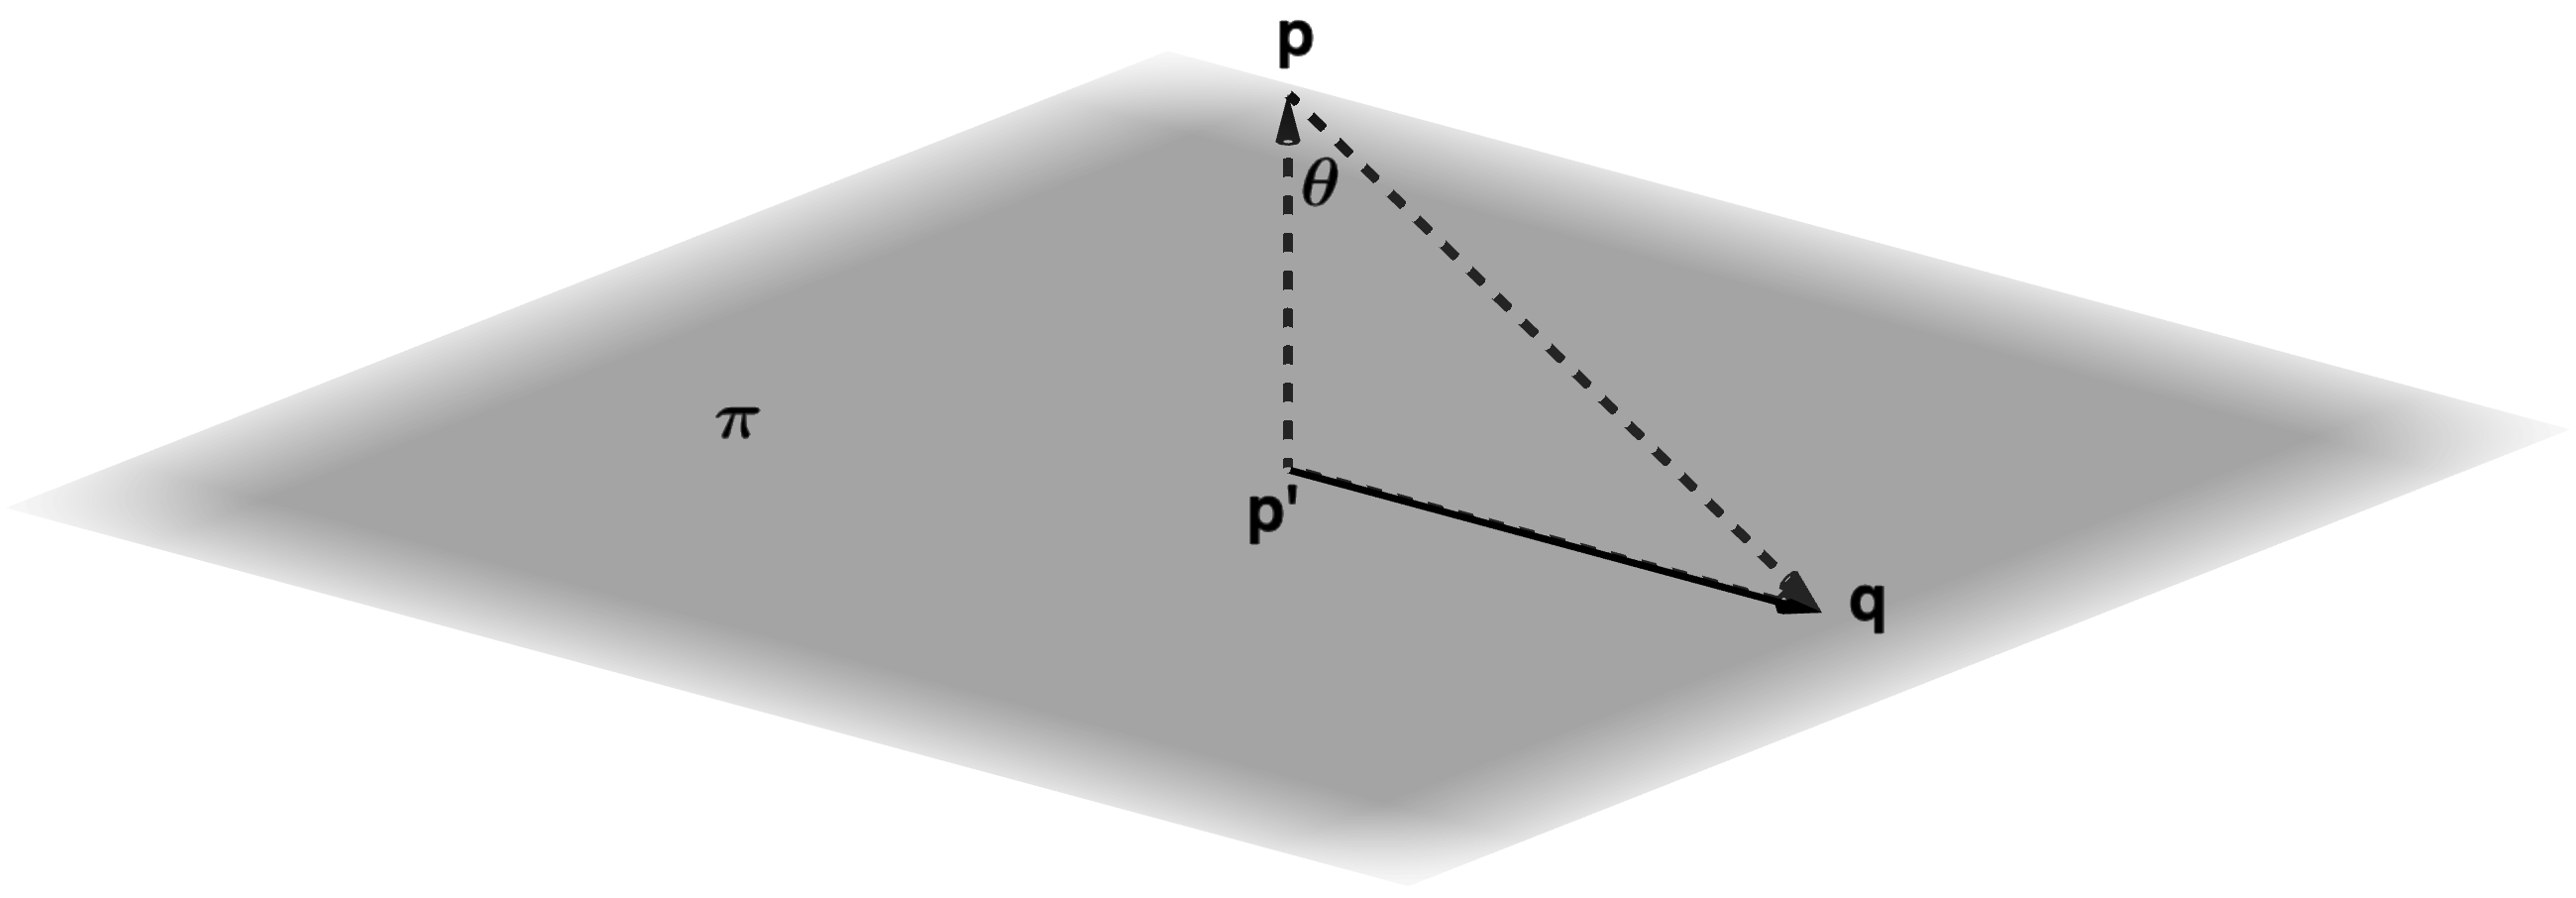
\includegraphics[width=11.4cm, height=4cm]{point-plane-distance}
            \begin{proof}
                Notice that the vertical line pointing towards $p$ is normal to the plane $\pi$, which means it is parallel to the normal vector $\mhat$, since both
                of them are orthogonal to the plane itself.
                Let's label the point at which the vertical line intercepts the plane as $p'$.\n
                Also, the length of the vertical line, $|\vec{pp'}|$ is indeed the distance between point $p$ and the plane $\pi$ -- the quantity
                we are looking for.\n
                If we take the angle $\theta$ between the vectors $\vec{pq}$ and the vertical line $\vec{pp'}$, the cosine of the angle is as follows:
                \begin{equation}
                    cos(\theta) = \frac{|\vec{pp'}|}{|\vec{pq}|}
                \end{equation}
                from the basic formula:
                \[cos(\theta) = \frac{adjacent}{hypotenuse}\]
                Then, if we take the dot product between the vectors $\vec{pq}$ and $\mhat$, we'll get:
                \[\vec{pq}\cdot\mhat = cos(\theta)|\vec{pq}||\mhat|\]
                which, if we rearrange yields,
                \begin{equation}
                    \frac{\vec{pq}\cdot\mhat}{|\vec{pq}||\mhat|} = cos(\theta)
                \end{equation}
                \bd{Notice: }The angle $\theta$ corresponds to the same angle in both equations $(12)$ and $(13)$ since $\mhat$ and $\vec{pp'}$ are parallel to each other, 
                thus are just multiples of the same vector.\n
                Therefore, if we equate equations $(12)$ and $(13)$, we get:
                \[\frac{|\vec{pp'}|}{|\vec{pq}|} = \frac{\vec{pq}\cdot\mhat}{|\vec{pq}||\mhat|}\]
                And crossing out the quantity $|\vec{pq}|$ from both sides:
                \[|\vec{pp'}| = \frac{\vec{pq}\cdot\mhat}{|\mhat|}\]
                If you realized, the numerator on the right hand side do not have an absolute value operator, although it should have one because the numerator
                needs to be strictly positive to yield a positive value for the distance of a line (distance is always positive in value, and denominator is already strictly positive).\n
                Thus our final equation is:
                \[\begin{split}
                    |\vec{pp'}| &= \frac{|\vec{pq}\cdot\mhat|}{|\mhat|}\n
                    dis(p, \pi) &= \frac{|\vec{pq}\cdot\mhat|}{|\mhat|}\qedhere
                \end{split}\]
                Which is indeed the point-to-plane-distance equation.
            \end{proof}
            \subsubsection{Example 1}
                Find the equation of a plane in scalar product form, passing through the point $q(2, 1, -3)$ and is perpendicular to $5i-2j+k$. What is the distance from the plane
                to the origin?\n
                \bd{Solution}\n
                Let $r = \begin{pmatrix} x \\ y \\ z \end{pmatrix}$, and $\mhat = \begin{pmatrix} 5 \\ -2 \\ 1 \end{pmatrix}$, then the plane has the Cartesian equation:
                \[r\cdot\mhat = d\]
                \begin{equation}
                    \begin{pmatrix} x\\y\\z \end{pmatrix} \cdot \begin{pmatrix} 5\-2\\1 \end{pmatrix} = d
                \end{equation}
                Then to find the value of $d$, we just need to substitute the vector $r$ by the coordinates of $q$:
                \[\begin{pmatrix}2\\1\\-3 \end{pmatrix} \cdot \begin{pmatrix} 5\\-2\\1 \end{pmatrix} = d\]
                \[10-2-3 = d\]
                \begin{equation}d = 5\end{equation}
                With that, our equation $(14)$ becomes
                \[\begin{pmatrix} x\\y\\z \end{pmatrix} \cdot \begin{pmatrix} 5\\-2\\1 \end{pmatrix} = 5\]
                And our Cartesian equation/scalar product is:
                \[5x -2y + z = 5\]
                To find the distance, we just need to utilize the equation we just derived at \bd{4.4 Distance from a Point to a Plane}:
                \[dis(O, \pi) = \frac{|\vec{OQ}\cdot\mhat|}{|\mhat|}\]
                Because the point is just the origin $O(0, 0, 0)$, the value of the numerator is equivalent to the value of $d$ in $(15)$.\n
                The only component we need to evaluate is the magnitude of $\mhat$:
                \[\begin{split}
                    |\mhat| &= \sqrt{(5)^2+(-2)^2+(1)^2}\\
                    |\mhat| &= \sqrt{30}
                \end{split}\]
                Finally, we can find the distance from origin to the plane as:
                \[\begin{split}
                    dis(O, \pi) &= \frac{|5|}{\sqrt{30}}\\
                    dis(O, \pi) &= \frac{5\sqrt{30}}{30}\\
                    dis(O, \pi) &= \frac{\sqrt{30}}{6}
                \end{split}\]
        
    \section{Angle}
        Like distance, the concept of angles will be used again in Pure Mathematics III, and also in a deeper level.
        \subsection{Angle between two Lines}
            As we know from one of the definitions of the dot product, the dot product can be used to find the angle in between two lines.
            \[cos(\theta) = \frac{a\cdot b}{|a||b|}\]
            At this point, you should be familiar with this, since it was used in Pure Mathematics I previously.
        
        \subsection{Angle between a Line and a Plane}
            The equation for this quantity is very similar to that of the angle between two lines. It is as follows:
            \[sin(\theta) = \frac{\nhat\cdot \mhat}{|\nhat||\mhat|}\]
            where $\theta$ is the angle between a line and a plane, $\nhat$ is the directional vector of the line, and
            $\mhat$ is the normal/orthogonal vector of the plane.\n
            It is also possible to find the angle by using the cosine function, as:
            \[cos\left(\frac{\pi}{2} - \theta\right) = sin(\theta)\]
            Therefore:
            \[\theta = \frac{\pi}{2} - \phi\]
            where,
            \[cos(\phi) = \frac{\nhat\cdot \mhat}{|\nhat||\mhat|}\]
            \subsubsection{Example 1}
                Find the angle between the line with the equation $r\cdot(2i+k) + \lambda(3i - 4j + k)$ and the plane with equation 
                $r\cdot(5i+j-6k) = 2$.\n
                \bd{Solution}\n
                We find that: 
                \[\begin{split}
                    \nhat &= \begin{pmatrix} 3 \\ -4 \\ 1 \end{pmatrix}\n
                    |\nhat| &= \sqrt{(3)^2 + (-4)^2 + (1)^2}\\
                    |\nhat| &= \sqrt{26}
                \end{split}\]
                and:
                \[\begin{split}
                    \mhat &= \begin{pmatrix} 5 \\ 1 \\ -6 \end{pmatrix}\n
                    |\mhat| &= \sqrt{(5)^2 + (1)^2 + (-6)^2}\\
                    |\mhat| &= \sqrt{62}
                \end{split}\]
                Then:
                \[\begin{split}
                    \nhat \cdot \mhat &= \begin{pmatrix} 3 \\ -4 \\ 1 \end{pmatrix} \cdot \begin{pmatrix} 5 \\ 1 \\ -6 \end{pmatrix}\\
                    \nhat \cdot \mhat &= 15 - 4 - 6\\
                    \nhat \cdot \mhat &= 5
                \end{split}\]
                With all the required values found, we can finally use the angle formula:
                \[\sin(\theta) = \frac{5}{\sqrt{26}\sqrt{62}}\]
                \[\begin{split}
                    \theta &= \sin^{-1}\left(\frac{5}{\sqrt{26}\sqrt{62}}\right)\\
                    \theta &\approx 7.2^{\circ}
                \end{split}\]

    \section{Past Paper Questions}
        \subsection{Problem 1}
            With respect to the origin $O$, the points $A$, $B$, $C$, $D$ have position vectors given by $\vec{OA} = i + 3j + 2k$,
            $\vec{OB} = 2i + j - k$, $\vec{OC} = 2i + 4j + k$, $\vec{OD} = -3i + j + 2k$.\n
            \bd{i) }Find the equation of the plane containing $A$, $B$ and $C$, giving your answer in the form $ax + by + cz = d$. \bd{[6]}\n
            \bd{ii) }The line through $D$ parallel to $\vec{OA}$ meets the plane with equation $x + 2y - z = 7$ at the point $P$. Find the
            position vector of $P$ and show that the length of $\vec{DP}$ is $2\sqrt{14}$. \bd{[5]}\n
            \bd{Solution}\n
            \bd{i) }Firstly, let's find two vectors parallel to the plane, namely $\vec{AB}$:
            \[\vec{AB} = (\vec{OB}) - (\vec{OA})\]
            \[\vec{AB} = \begin{pmatrix} 2\\1\\-1 \end{pmatrix} - \begin{pmatrix} 1\\3\\2 \end{pmatrix}\]
            \[\vec{AB} = \begin{pmatrix} 1\\-2\\-3 \end{pmatrix}\]
            and $\vec{AC}$:
            \[\vec{AC} = (\vec{OC}) - (\vec{OA})\]
            \[\vec{AC} = \begin{pmatrix} 2\\4\\1 \end{pmatrix} - \begin{pmatrix} 1\\3\\2 \end{pmatrix}\]
            \[\vec{AC} = \begin{pmatrix} 1\\1\\-1 \end{pmatrix}\]
            With those two vectors, we can find the vector equation of the plane:
            \[r = \vec{OA} + \lambda (\vec{AB}) + \mu (\vec{AC})\]
            \[\begin{split}
                r &= \begin{pmatrix} 1\\3\\2 \end{pmatrix} + \lambda \begin{pmatrix} 1\\-2\\-3 \end{pmatrix} + \mu \begin{pmatrix} 1\\1\\-1 \end{pmatrix}\\
                r &= \begin{pmatrix} 1 + \lambda + \mu \\ 3 -2\lambda +\mu \\ 2 -3\lambda -\mu \end{pmatrix}   
            \end{split}\]
            Then, we need to find a vector orthogonal to the plane, which we can find by the cross product between $\vec{AB}$ and $\vec{AC}$:
            \begin{center}
                \begin{tabular}{|c || c | c | c|} 
                \hline
                Vector & $i$ & $j$ & $k$ \\
                \hline
                $\vec{AB}$ & $1$ & $-2$ & $-3$ \\ 
                \hline
                $\vec{AC}$ & $1$ & $1$ & $-1$ \\
                \hline
               \end{tabular}
            \end{center}
            \[\begin{split}
                \thus\vec{AB}\times\vec{AC} &= (2+3)i - (-1+3)j + (1+2)k\\
                \vec{AB}\times\vec{AC} &= 5i - 2j + 3k\\
                \vec{AB}\times\vec{AC} &= \begin{pmatrix} 5 \\ -2 \\ 3 \end{pmatrix} = \mhat
            \end{split}\]
            Finally to find the Cartesian equation of the plane:
            \[\begin{split}
                r \cdot \mhat &= (\vec{OA)} \cdot \mhat\\
                \begin{pmatrix} x \\ y \\ z \end{pmatrix} \cdot \begin{pmatrix} 5 \\ -2 \\ 3 \end{pmatrix} &= \begin{pmatrix} 1 \\ 3 \\ 2 \end{pmatrix} \cdot \begin{pmatrix} 5 \\ -2 \\ 3 \end{pmatrix}\\
                5x - 2y + 3z &= 5 - 6 + 6
            \end{split}\]
            Obtaining:
            \[5x - 2y + 3z = 5\]
            as our Cartesian equation of the plane.\n
            \bd{ii) } We need to first find the vector equation of the line, which is quite simple. Since the line passes through $D$ and is parallel to $\vec{OA}$,
            we can immediately find:
            \[r = \vec{OD} + \lambda (\vec{OA})\]
            \[\begin{split}
                \begin{pmatrix} x \\ y \\ z \end{pmatrix} &= \begin{pmatrix} -3 \\ 1 \\ 2 \end{pmatrix} + \lambda \begin{pmatrix} 1 \\ 3 \\ 2 \end{pmatrix}\\
                \begin{pmatrix} x \\ y \\ z \end{pmatrix} &= \begin{pmatrix} -3 + \lambda \\ 1 + 3\lambda \\ 2 + 2\lambda \end{pmatrix}    
            \end{split}\]
            From which we can find the set of parametric equations:
            \begin{equation}
                \begin{split}
                    x &= -3 + \lambda\\
                    y &= 1 + 3\lambda\\
                    z &= 2 + 2\lambda
                \end{split}
            \end{equation}
            Then, to find the point of intersection of the line and the plane, we need to find the value of $\lambda$ whose coordinates satisfies the plane equation:
            \[x + 2y - z = 7\]
            Substituting the variables with the ones obtained in $(16)$ yields:
            \[(-3 + \lambda) + 2(1 + 3\lambda) - (2 + 2\lambda) = 7\]
            \[-3 + \lambda + 2 + 6\lambda - 2 - 2\lambda = 7\]
            \[5\lambda = 10\]
            \[\lambda = 2\]
            Thus, the coordinates of the point $P$ is just the respective values in $(16)$ with the value of $\lambda$ being $2$:
            \[\begin{split}
                P &= \begin{pmatrix} -3 + 2 \\ 1 + 6 \\ 2 + 4 \end{pmatrix}\\
                P &= \begin{pmatrix} -1 \\ 7 \\ 6 \end{pmatrix}
            \end{split}\]
            Lastly, the vector $\vec{DP}$:
            \[\vec{DP} = P - (\vec{OD})\]
            \[\vec{DP} = \begin{pmatrix} -1 \\ 7 \\ 6 \end{pmatrix} - \begin{pmatrix} -3 \\ 1 \\ 2 \end{pmatrix}\]
            \[\vec{DP} = \begin{pmatrix} 2 \\ 6 \\ 4 \end{pmatrix}\]
            And its magnitude:
            \[\begin{split}
                |\vec{DP}| &= \sqrt{(2)^2 + (6)^2 + (4)^2}\\
                |\vec{DP}| &= \sqrt{56}\\
                |\vec{DP}| &= \sqrt{4 * 14}\\
                |\vec{DP}| &= 2\sqrt{14}
            \end{split}\]
            which is equivalent to what the question required from us.

        \subsection{Problem 2}
            The points $A$ and $B$ have position vectors, relative to the origin $O$, given by $\vec{OA} = i + j + k$ and $\vec{OB} = 2i + 3k$.
            The line $l$ has vector equation $r = 2i - 2j - k + \mu(-i + 2j + k)$.\n
            \bd{i) }Show that the line passing through $A$ and $B$ does not intersect $l$. \bd{[4]}\n
            \bd{ii) }Show that the length of the perpendicular from $A$ to $l$ is $\frac{1}{\sqrt{2}}$. \bd{[5]}.\n
            \bd{Solution}\n
            \bd{i) }To find the vector equation of the line passing through points $A$ and $B$, we need to find its directional vector $\vec{AB}$:
            \[\begin{split}
                \vec{AB} &= \vec{OB} - \vec{OA} \\
                \vec{AB} &= \begin{pmatrix} 2 \\ 0 \\ 3 \end{pmatrix} - \begin{pmatrix} 1 \\ 1 \\ 1 \end{pmatrix}\\
                \vec{AB} &= \begin{pmatrix} 1 \\ -1 \\ 2 \end{pmatrix}
            \end{split}\]
            With that, we can find the vector equation of the line that passes through points $A$ and $B$, which we'll denote with $s$:
            \[\begin{split}
                s &= \vec{OA} + \lambda (\vec{AB})\\
                s &= \begin{pmatrix} 1 \\ 1 \\ 1 \end{pmatrix} + \lambda \begin{pmatrix} 1 \\ -1 \\ 2 \end{pmatrix}
            \end{split}\]
            Then, to check whether the lines do not intersect, we can equate the vector equations $r$ and $s$:
            \[\begin{split}
                r &= s\\
                \begin{pmatrix} 2 \\ -2 \\ -1 \end{pmatrix} + \mu\begin{pmatrix} -1 \\ 2 \\ 1 \end{pmatrix} &= \begin{pmatrix} 1 \\ 1 \\ 1 \end{pmatrix} + \lambda \begin{pmatrix} 1 \\ -1 \\ 2 \end{pmatrix}\\
                \begin{pmatrix} 2 - \mu \\ -2 + 2\mu \\ -1 + \mu\end{pmatrix} &= \begin{pmatrix} 1 + \lambda \\ 1  - \lambda\\ 1 + 2\lambda \end{pmatrix}    
            \end{split}\]
            From there, we obtain a system of linear equations, as the following:
            \begin{equation}
                \begin{split}
                    2 - \mu &= 1 + \lambda\\
                    \thus \lambda + \mu &= 1
                \end{split}
            \end{equation}
            \begin{equation}
                \begin{split}
                    -2 + 2\mu &= 1  - \lambda\\
                    \thus \lambda + 2\mu &= 3
                \end{split}
            \end{equation}
            If we subtract equation $(18)$ with equation $(17)$, we find that:
            \[\mu = 2\]
            and
            \[\lambda = -1\]
            With both of these values found, we can check whether they are consistent if we substitute the scalars in equations $r$ and $s$ respectively.
            \[\begin{split}
                \begin{pmatrix} 2 - 2 \\ -2 + 4 \\ -1 + 2\end{pmatrix} &\overset{?}{=} \begin{pmatrix} 1 - 1 \\ 1  + 1\\ 1 - 2 \end{pmatrix}\\
                \begin{pmatrix} 0 \\ 2 \\ 1\end{pmatrix} &\overset{?}{=} \begin{pmatrix} 0 \\ 2\\ -1 \end{pmatrix}\\
                \begin{pmatrix} 0 \\ 2 \\ 1\end{pmatrix} &\neq \begin{pmatrix} 0 \\ 2\\ -1 \end{pmatrix}
            \end{split}\]
            Since the values of $\lambda$ and $\mu$ are inconsistent, therefore there are no points of intersection between the lines -- which is what
            the question required us to show.\n
            \bd{ii) }We are going to use the intuitive method shown in \bd{4.2.1 Example 1}.\n
            Let $A'$ be the foot of the perpendicular from point $A$ to the line $l$. Since $A'$ lies on line $l$, then $A'$ has the general equation:
            \[\begin{split}
                A' &= \begin{pmatrix} 2 \\ -2 \\ -1 \end{pmatrix} + \mu \begin{pmatrix} -1 \\ 2 \\ 1 \end{pmatrix}\\
                A' &= \begin{pmatrix} 2-\mu \\ -2+2\mu \\ -1+\mu \end{pmatrix}
            \end{split}\]
            Then, we find the vector that passes through lines $A$ and $A'$, namely $\vec{AA'}$:
            \[\begin{split}
                \vec{AA'} &= A' - A\\
                \vec{AA'} &= \begin{pmatrix} 2-\mu \\ -2+2\mu \\ -1+\mu \end{pmatrix} - \begin{pmatrix} 1 \\ 1 \\ 1 \end{pmatrix}\\
                \vec{AA'} &= \begin{pmatrix} 1-\mu \\ -3+2\mu \\ -2+\mu \end{pmatrix}
            \end{split}\]
            As we know, $\vec{AA'}$ is perpendicular to $\nhat$, the directional vector of line $l$. Thus:
            \begin{equation}
                (\vec{AA'}) \cdot \nhat = 0
            \end{equation}
            If we can find the value of $\mu$ that satisfies equation $(19)$, we can then find the magnitude of $\vec{AA'}$, which is the length of the perpendicular
            from $A$ to $l$.
            \[\begin{split}
                \begin{pmatrix} 1-\mu \\ -3+2\mu \\ -2+\mu \end{pmatrix} \cdot \begin{pmatrix} -1 \\ 2 \\ 1 \end{pmatrix} &= 0\\
                -1 + \mu - 6 + 4\mu - 2 + \mu &= 0\\
                6\mu &= 9\\
                \mu &= \frac{3}{2}
            \end{split}\]
            With the value of $\mu$ found, we can substitute its value to the vector $\vec{AA'}$:
            \[\begin{split}
                \vec{AA'} &= \begin{pmatrix} 1-\frac{3}{2} \\ -3+3 \\ -2+\frac{3}{2} \end{pmatrix}\\
                \vec{AA'} &= \begin{pmatrix} -\frac{1}{2} \\ 0 \\ -\frac{1}{2} \end{pmatrix}
            \end{split}\]
            Lastly, we only need to find its magnitude:
            \[\begin{split}
                |\vec{AA'}| &= \sqrt{\left(-\frac{1}{2}\right)^ 2 + (0)^2 + \left(-\frac{1}{2}\right)^ 2}\\
                |\vec{AA'}| &= \sqrt{\frac{1}{4} + \frac{1}{4}}\\
                |\vec{AA'}| &= \sqrt{\frac{1}{2}}\\
                |\vec{AA'}| &= \frac{1}{\sqrt{2}}
            \end{split}\]
            which is equivalent to what the question required us to show.
        \subsection{Problem 3}
            The line $l$ has equation $r = i + j + k + \lambda(ai + 2j + k)$, where $a$ is a constant. The plane $p$ has equation
            $x + 2y + 2z = 6$. Find the value or values of $a$ in each of the following cases.\n
            \bd{i) }The line $l$ is parallel to the plane $p$. \bd{[2]}\n
            \bd{ii) }The line $l$ intersects the line passing through the points with position vectors $3i + 2j + k$ and $i + j - k$. \bd{[4]}\n
            \bd{iii) }The acute angle between the line $l$ and the plane $p$ is $tan^{-1}(2)$. \bd{[5]}\n
            \bd{Solution}\n
            \bd{i) }Let $\nhat$ be the directional vector of the line $l$, such that:
            \[\nhat = \begin{pmatrix} a \\ 2 \\ 1 \end{pmatrix}\]
            And $\mhat$ be the normal vector to the plane $p$:
            \[\mhat = \begin{pmatrix} 1 \\ 2 \\ 2 \end{pmatrix}\]
            If given that the line $l$ is parallel to the plane $p$, then $\nhat$ would be orthogonal to the normal vector $\mhat$, since both the line
            and the plane are normal to the vector $\mhat$. Thus the equation:
            \[\nhat \cdot \mhat = 0\]
            must be satisfied. Therefore:
            \[\begin{split}
                \begin{pmatrix} a \\ 2 \\ 1 \end{pmatrix} \cdot \begin{pmatrix} 1 \\ 2 \\ 2 \end{pmatrix} &= 0\\
                a + 4 + 2 &= 0
            \end{split}\]
            Finally,
            \[a = -6\]
            \bd{ii) }We need to first find the equation of the line that passes through both position vectors given by the problem, which we'll denote with $s$.
            \[\begin{split}
                s &= \begin{pmatrix} 3 \\ 2 \\ 1 \end{pmatrix} + \mu \begin{pmatrix} 3 - 1 \\ 2 - 1 \\ 1 - (-1) \end{pmatrix}\\
                s &= \begin{pmatrix} 3 \\ 2 \\ 1 \end{pmatrix} + \mu \begin{pmatrix} 2 \\ 1 \\ 2 \end{pmatrix}\\
                s &= \begin{pmatrix} 3 + 2\mu \\ 2 + \mu \\ 1 + 2\mu \end{pmatrix}
            \end{split}\]
            Then to find the point of intersection, we need to equate $r$ to $s$ and find the values of $\mu$ and $\lambda$ that satisfy the system of linear equations.
            \[\begin{split}
                r &=s\\
                \begin{pmatrix} 1 + a\lambda \\ 1 + 2\lambda \\ 1 + \lambda \end{pmatrix} &= \begin{pmatrix} 3 + 2\mu \\ 2 + \mu \\ 1 + 2\mu \end{pmatrix}
            \end{split}\]
            Assuming the point of intersection exists, we can solve the following system:
            \begin{equation}
                \begin{split}
                    1 + 2\lambda &= 2 + \mu\\
                    1 + \lambda &= 1 + 2\mu
                \end{split}
            \end{equation}
            Manipulating the second equation above yields:
            \[\begin{split}
                1 + \lambda &= 1 + 2\mu\\
                \thus \lambda &= 2 \mu
            \end{split}\]
            From which we can plug into the first equation.
            \[\begin{split}
                1 + 2(2\mu) &= 2 + \mu\\
                1 + 4\mu &= 2 + \mu\\
                3\mu &= 1\\
                \mu &= \frac{1}{3}
            \end{split}\]
            Then we can find the value of $\lambda$:
            \[\begin{split}
                \lambda &= 2 \mu\\
                \lambda &= 2 \left(\frac{1}{3}\right)\\
                \lambda &= \frac{2}{3}
            \end{split}\]
            With the initial assumption that the system is indeed consistent, we can finally solve for the value of $a$,
            \[\begin{split}
                1 + a \lambda &= 3 + 2\mu\\
                1 + a \left(\frac{2}{3}\right) &= 3 + 2 \left(\frac{1}{3}\right)\\
                \frac{2a}{3} &= 2 + \frac{2}{3}\\
                \frac{2a}{3} &= \frac{8}{3}\\
                a &= \frac{8}{2}\\
                a &= 4
            \end{split}\]
            \bd{iii) }We know that the angle between a line and a plane is given by the equation:
            \[sin(\theta) = \frac{\nhat\cdot\mhat}{|\nhat||\mhat|}\]
            where $\nhat$ is the directional vector of the line and $\mhat$ is the normal vector of the plane.\\
            Firstly, we need to find each of the respective components, namely:
            \[\nhat = \begin{pmatrix} a \\ 2 \\ 1 \end{pmatrix}\]
            and its magnitude:
            \[\begin{split}
                |\nhat| &= \sqrt{a^2 + 4 + 1}\\
                |\nhat| &= \sqrt{a^2 + 5}
            \end{split}\]
            Then the normal vector of the plane:
            \[\mhat = \begin{pmatrix} 1 \\ 2 \\ 2 \end{pmatrix}\]
            and its magnitude:
            \[\begin{split}
                |\mhat| &= \sqrt{1 + 4 + 4}\\
                |\mhat| &= \sqrt{9}\\
                |\mhat| &= 3
            \end{split}\]
            The dot product of the two vectors yields:
            \[\begin{split}
                \nhat \cdot \mhat &= \begin{pmatrix} a \\ 2 \\ 1 \end{pmatrix} \cdot \begin{pmatrix} 1 \\ 2 \\ 2 \end{pmatrix}\\
                \nhat \cdot \mhat &= a + 4 + 2\\
                \nhat \cdot \mhat &= a + 6
            \end{split}\]
            With all the components found, we can find an expression of the angle, such that:
            \begin{equation}sin(\theta) = \frac{a + 6}{3\sqrt{a^2 + 5}}\end{equation}
            Given from the problem, we also know that the angle is also equal to $tan^{-1}(2)$.
            \begin{equation}
                \begin{split}
                    \theta &= tan^{-1}(2)\\
                    tan(\theta) &= 2
                \end{split}
            \end{equation}
            We should somehow correlate the quantities $(21)$ and $(22)$. Sure we can take the value of $\theta$ as the decimal approximation
            of equation $(22)$, but it won't give an exact answer -- which is preferable. This is when trigonometric identities get in handy.\n
            \bd{Recall}:
            \[cot^{2}(\theta) + 1 = csc^{2}(\theta)\]
            which we can express as:
            \[\left(\frac{1}{tan(\theta)}\right)^2 + 1 = \left(\frac{1}{sin(\theta)}\right)^2\]
            Therefore, using equations $(21)$ and $(22)$, we obtain:
            \[\begin{split}
                \left(\frac{1}{2}\right)^2 + 1 &= \left(\frac{3\sqrt{a^2 + 5}}{a+6}\right)^2\n
                \frac{1}{4} + 1 &= \frac{9(a^2 + 5)}{a^2 + 12a + 36}\n
                \frac{5}{4} &= \frac{9a^2 + 45}{a^2 + 12a + 36}\n
                5a^2 + 60a + 180 &= 36a^2 + 180\\
                0 &= 31a^2 - 60a
                % 0 &= a(31a - 60)
            \end{split}\]
            Finding the zeroes of the equation above will yield the values of $a$. We can do this by factoring $a$.
            \[0 = a(31a - 60)\]
            Obtaining the values of $a$ such that:
            \[a = 0\]
            and
            \[\begin{split}
                0 &= 31a - 60\\
                31a &= 60\\
                a &= \frac{60}{31}
            \end{split}\]
    \bibliographystyle{apacite}
    \bibliography{References}
\end{document}